\documentclass{article}
\usepackage{amsmath}
\usepackage{amsfonts}
\usepackage{geometry}
\usepackage{booktabs}
\usepackage{tcolorbox}
\usepackage{tikz}
\usetikzlibrary{arrows.meta, patterns, positioning}

\geometry{a4paper, margin=1in}

\begin{document}

\title{Momentum and Impulse}
\author{}
\date{}
\maketitle

\section{Introduction: The Egg Drop Hook}
Consider tossing an egg against a brick wall versus tossing it into a sagging bedsheet with the same initial speed.
\begin{itemize}
    \item \textbf{Brick Wall:} The egg stops abruptly ($\Delta t$ is extremely small). The wall exerts a huge force, shattering the egg.
    \item \textbf{Bedsheet:} The egg stops gradually ($\Delta t$ is large). The sheet exerts a much smaller force, leaving the egg intact.
\end{itemize}
In both cases, the egg's initial velocity is $v$, and its final velocity is $0$. Thus, its change in velocity ($\Delta v$) and its mass ($m$) are the same. This leads us to define a new physical quantity: \textbf{Momentum}.

\section{Momentum ($\vec{p}$)}
Momentum is defined as the product of an object's mass and its velocity. It is a vector quantity, meaning it has both magnitude and direction.

\begin{equation}
\vec{p} = m\vec{v}
\end{equation}

Where:
\begin{itemize}
    \item $\vec{p}$ is the \textbf{momentum}, measured in kilogram-meters per second ($\text{kg} \cdot \text{m/s}$).
    \item $m$ is the \textbf{mass}, measured in kilograms ($\text{kg}$).
    \item $\vec{v}$ is the \textbf{velocity}, measured in meters per second ($\text{m/s}$).
\end{itemize}
\textbf{Note:} The momentum vector $\vec{p}$ always points in the same direction as the velocity vector $\vec{v}$.

\section{Impulse ($\vec{J}$) and the Impulse-Momentum Theorem}
To change an object's momentum, a net force must be applied over a period of time. This product of force and time is called \textbf{Impulse}.

\begin{equation}
\vec{J} = \vec{F}_{\text{avg}}\Delta t
\end{equation}

By starting with Newton's Second Law ($\vec{F}_{\text{net}} = m\vec{a}$) and remembering that $\vec{a} = \frac{\Delta \vec{v}}{\Delta t}$, we can derive the \textbf{Impulse-Momentum Theorem}:

\begin{equation}
\vec{J} = \Delta\vec{p} = \vec{p}_f - \vec{p}_i = m\vec{v}_f - m\vec{v}_i
\end{equation}

\subsection{Graphical Representation: Force vs. Time}
A core concept in AP Physics 1 is analyzing the Force vs. Time ($F-t$) graph.
\begin{itemize}
    \item The \textbf{area under the curve} of a Force vs. Time graph represents the \textbf{Impulse} ($\vec{J}$), which is equal to the change in momentum ($\Delta \vec{p}$).
    \item Real-world collision forces are not constant. They often form a "bell-shaped" curve. 
\end{itemize}

\begin{figure}[h]
    \centering
    \begin{minipage}{0.45\textwidth}
        \centering
        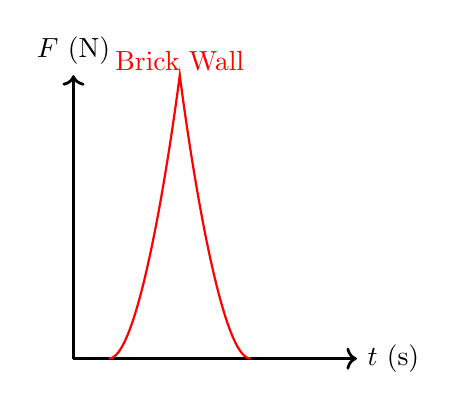
\begin{tikzpicture}[scale=0.9, line width=1pt]
            % Axes
            \draw[->] (0,0) -- (4,0) node[right] {$t$ (s)};
            \draw[->] (0,0) -- (0,4) node[above] {$F$ (N)};
            
            % Curve A (Brick wall)
            \draw[color=red, thick] (0.5,0) .. controls (1,0) and (1.5,4) .. (1.5,4)
                                          .. controls (1.5,4) and (2,0) .. (2.5,0);
            
            \node[red] at (1.5, 4.2) {Brick Wall};
        \end{tikzpicture}
        
        \vspace{0.2cm}
        \small (a) Large peak force, short time (Small $\Delta t$)
    \end{minipage}%
    \hfill
    \begin{minipage}{0.45\textwidth}
        \centering
        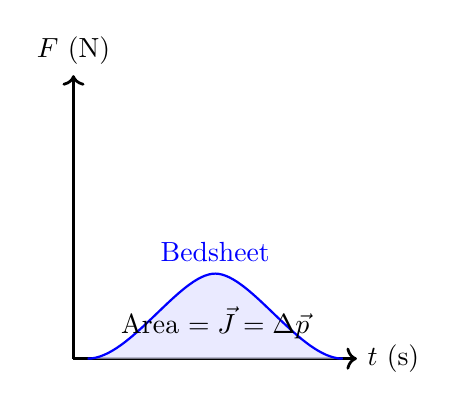
\begin{tikzpicture}[scale=0.9, line width=1pt]
            % Axes
            \draw[->] (0,0) -- (4,0) node[right] {$t$ (s)};
            \draw[->] (0,0) -- (0,4) node[above] {$F$ (N)};
            
            % Area under curve
            \fill[blue!10, opacity=0.8] (0.2,0) .. controls (0.8,0) and (1.5,1.2) .. (2,1.2)
                                           .. controls (2.5,1.2) and (3.2,0) .. (3.8,0) -- cycle;
            
            % Curve B (Bedsheet)
            \draw[color=blue, thick] (0.2,0) .. controls (0.8,0) and (1.5,1.2) .. (2,1.2)
                                           .. controls (2.5,1.2) and (3.2,0) .. (3.8,0);
            
            \node[blue] at (2, 1.5) {Bedsheet};
            \node at (2, 0.5) {Area $= \vec{J} = \Delta\vec{p}$};
        \end{tikzpicture}
        
        \vspace{0.2cm}
        \small (b) Smaller peak force, longer time (Large $\Delta t$)
    \end{minipage}
    \caption{The two graphs have the \textbf{same area} (same change in momentum), but drastically different maximum peak forces.}
\end{figure}

\section{The Vector Nature: Bouncing vs. Sticking}
In AP Physics, \textbf{direction matters}! Always assign a positive and negative direction to your velocities.
Consider a ball of mass $m$ thrown at a wall with a speed $v$ (let moving to the right be positive).

\begin{tcolorbox}[colback=gray!10, colframe=black, title=Comparison: Bouncing vs Sticking]
    \textbf{Case 1: The ball sticks to the wall (Inelastic)}
    \begin{itemize}
        \item Initial momentum: $\vec{p}_i = +mv$
        \item Final momentum: $\vec{p}_f = 0$
        \item Change in momentum: $\Delta \vec{p} = \vec{p}_f - \vec{p}_i = 0 - mv = -mv$
    \end{itemize}
    
    \vspace{0.3cm}
    \textbf{Case 2: The ball bounces back elastically (Elastic)}
    \begin{itemize}
        \item Initial momentum: $\vec{p}_i = +mv$
        \item Final momentum: $\vec{p}_f = -mv$ (moving in the opposite direction!)
        \item Change in momentum: $\Delta \vec{p} = \vec{p}_f - \vec{p}_i = (-mv) - (+mv) = -2mv$
    \end{itemize}
\end{tcolorbox}
\textbf{Conclusion:} Bouncing produces \textbf{twice} the change in momentum (and thus delivers twice the impulse to the wall) as sticking!

\section{Conservation of Momentum}
Newton's Third Law states that forces come in equal and opposite pairs. If two objects, A and B, collide, the force that A exerts on B is equal and opposite to the force B exerts on A:
\begin{equation}
\vec{F}_{\text{A on B}} = -\vec{F}_{\text{B on A}}
\end{equation}

Since the time of the collision ($\Delta t$) must be exactly the same for both objects, the impulses they deliver to each other are also equal and opposite:
\begin{equation}
\vec{J}_{\text{A on B}} = -\vec{J}_{\text{B on A}}
\end{equation}

Applying the Impulse-Momentum Theorem ($\vec{J} = \Delta\vec{p}$):
\begin{equation}
\Delta\vec{p}_{\text{B}} = -\Delta\vec{p}_{\text{A}} \implies \Delta\vec{p}_{\text{A}} + \Delta\vec{p}_{\text{B}} = 0
\end{equation}
This means the \textbf{total change in momentum of the two-object system is zero}. 

\begin{tcolorbox}[colback=blue!5, colframe=blue!40!black, title=Law of Conservation of Momentum]
In an isolated system (where the net external force is zero), the total momentum of the system remains constant before, during, and after any interaction (like a collision or an explosion).
\begin{equation}
\Sigma \vec{p}_i = \Sigma \vec{p}_f
\end{equation}
For a two-object collision:
\begin{equation}
m_1\vec{v}_{1i} + m_2\vec{v}_{2i} = m_1\vec{v}_{1f} + m_2\vec{v}_{2f}
\end{equation}
\end{tcolorbox}

\subsection{Defining the System (AP Key Concept)}
Whether momentum is considered "conserved" depends entirely on \textbf{how you define your system}.
\begin{itemize}
    \item \textbf{Open System:} Exists when net external forces (like friction, or a hand pushing) act on the objects. The momentum of an open system \textbf{changes}. This change is equal to the external impulse ($\vec{J}_{\text{ext}} = \Delta\vec{p}_{\text{sys}}$).
    \item \textbf{Isolated (Closed) System:} Exists when there are no net external forces. For example, two ice skaters pushing off each other on frictionless ice. Because the push is an \emph{internal} force between the two parts of the system, the total momentum of the "Skater 1 + Skater 2" system is conserved.
\end{itemize}

\newpage
\section{Typical AP Example Problems}

\subsection*{Example 1: Graphical Analysis of Impulse (F-t Graph)}
\textbf{Problem:} A horizontally moving $2.0 \text{ kg}$ cart is initially moving to the right at $3.0 \text{ m/s}$. It collides with a force sensor that applies a varying force to the left. The force vs. time graph of the collision is shown below as a triangle with a peak force of $20 \text{ N}$ lasting for $0.5 \text{ s}$. What is the final velocity of the cart after the collision?

\vspace{0.2cm}
\begin{center}
    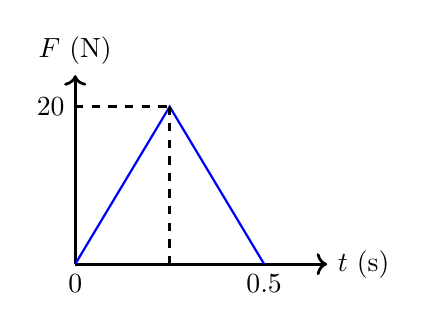
\begin{tikzpicture}[scale=0.8, line width=1pt]
        \draw[->] (0,0) -- (4,0) node[right] {$t$ (s)};
        \draw[->] (0,0) -- (0,3) node[above] {$F$ (N)};
        \draw[thick, blue] (0,0) -- (1.5,2.5) -- (3,0);
        \node[left] at (0, 2.5) {20};
        \node[below] at (3, 0) {0.5};
        \node[below] at (0, 0) {0};
        \draw[dashed] (0,2.5) -- (1.5,2.5);
        \draw[dashed] (1.5,0) -- (1.5,2.5);
    \end{tikzpicture}
\end{center}

\vspace{0.2cm}
\textbf{Solution:}

\vspace{5cm}

\subsection*{Example 2: Bouncing vs. Sticking}
\textbf{Problem:} Toy car A ($m = 0.5 \text{ kg}$) and toy car B ($m = 0.5 \text{ kg}$) are both moving to the right at $4.0 \text{ m/s}$. Car A hits a sticky putty wall and comes to a complete stop. Car B hits a bouncy spring wall and rebounds to the left at $3.0 \text{ m/s}$. Which car experiences the greater magnitude of impulse, and by how much?

\textbf{Solution:}

\vspace{4.5cm}

\subsection*{Example 3: Defining the System (Conceptual FRQ Style)}
\textbf{Problem:} An astronaut is floating stationary in space relative to her spaceship. She throws a heavy wrench away from the ship. 
\begin{itemize}
    \item[(a)] If the system is defined as just the astronaut, is momentum conserved? Explain.
    \item[(b)] If the system is defined as the astronaut and the wrench, is momentum conserved? Explain.
\end{itemize}

\textbf{Solution:}

\vspace{3.5cm}

\subsection*{Example 4: 1D Inelastic Collision}
\textbf{Problem:} A skater of mass $60 \text{ kg}$ is gliding to the right at $4.0 \text{ m/s}$. He catches a $10 \text{ kg}$ medicine ball that was thrown horizontally towards him (to the left) at $5.0 \text{ m/s}$. What is the velocity of the skater-ball system immediately after the catch?

\textbf{Solution:}

\vspace{5cm}

\subsection*{Example 5: An "Explosion" (Separation) Problem}
\textbf{Problem:} Two carts on a frictionless track, Cart A ($m = 1.0 \text{ kg}$) and Cart B ($m = 3.0 \text{ kg}$), are initially at rest and pushed together, compressing a spring between them. They are released, and the spring pushes them apart. If Cart A shoots off to the left at a speed of $6.0 \text{ m/s}$, what is the final velocity (magnitude and direction) of Cart B?

\textbf{Solution:}

\vspace{4.5cm}

\subsection*{Example 6: Evaluating System Momentum (Conceptual)}
\textbf{Problem:} A block slides down a curved, frictionless ramp. 
\begin{itemize}
    \item[(a)] If the system is defined as just the block, is the magnitude of the block's momentum conserved? Why or why not?
    \item[(b)] If the system is defined as the block and the Earth, is the total momentum of this system conserved? Why or why not?
\end{itemize}

\textbf{Solution:}

\vspace{4.5cm}

\end{document}
